%! TEX encoding = utf8
\chapter{Odpowiedzi skokowe}

Rozważamy punkt pracy oraz 6 różnych wartości skoku, z zera do: $-0,5$, $-0,25$, $0,25$, $0,5$, $0,75$, $1,0$.

\section{Opowiedzi skokowe}

\begin{figure}[H]
\centering
% This file was created by matlab2tikz.
%
%The latest updates can be retrieved from
%  http://www.mathworks.com/matlabcentral/fileexchange/22022-matlab2tikz-matlab2tikz
%where you can also make suggestions and rate matlab2tikz.
%
\definecolor{mycolor1}{rgb}{0.00000,0.44700,0.74100}%
\definecolor{mycolor2}{rgb}{0.85000,0.32500,0.09800}%
\definecolor{mycolor3}{rgb}{0.92900,0.69400,0.12500}%
\definecolor{mycolor4}{rgb}{0.49400,0.18400,0.55600}%
\definecolor{mycolor5}{rgb}{0.46600,0.67400,0.18800}%
\definecolor{mycolor6}{rgb}{0.30100,0.74500,0.93300}%
%
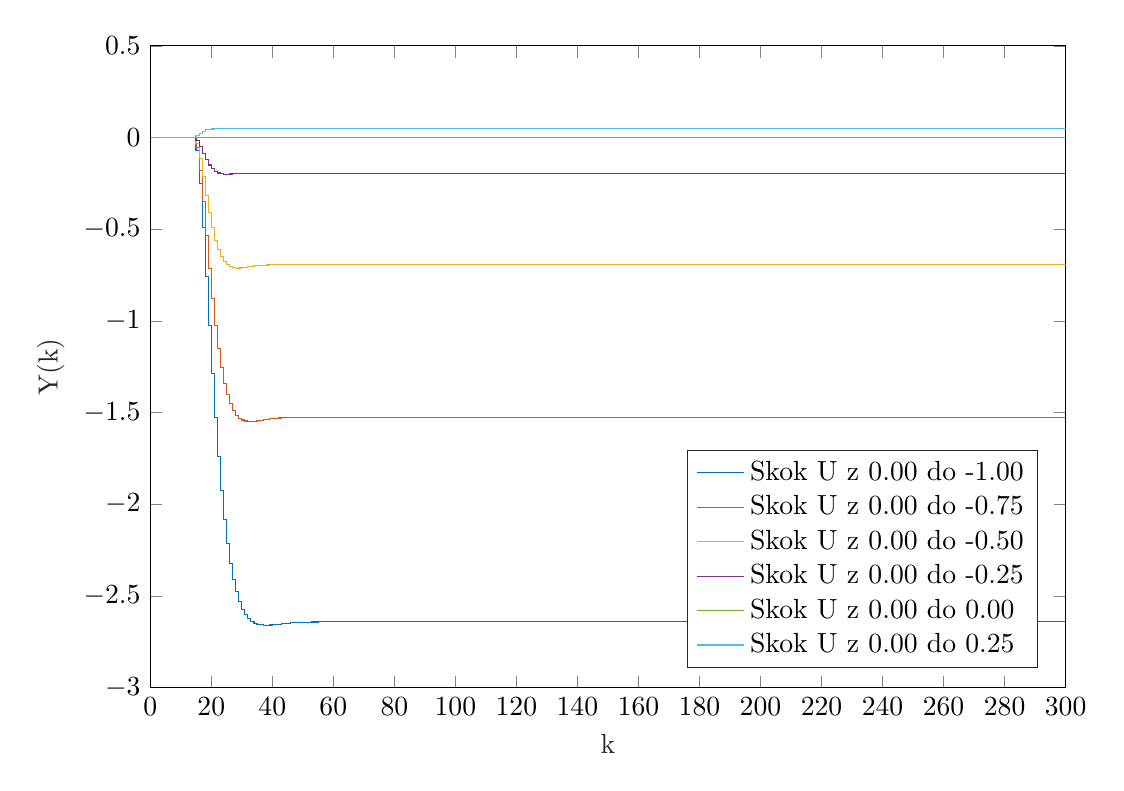
\begin{tikzpicture}

\begin{axis}[%
width=4.577in,
height=3.209in,
at={(0.768in,0.433in)},
scale only axis,
xmin=0,
xmax=300,
xlabel style={font=\color{white!15!black}},
xlabel={k},
ymin=-3,
ymax=0.5,
ylabel style={font=\color{white!15!black}},
ylabel={Y(k)},
axis background/.style={fill=white},
legend style={at={(0.97,0.03)}, anchor=south east, legend cell align=left, align=left, draw=white!15!black}
]
\addplot[const plot, color=mycolor1] table[row sep=crcr] {%
1	0\\
2	0\\
3	0\\
4	0\\
5	0\\
6	0\\
7	0\\
8	0\\
9	0\\
10	0\\
11	0\\
12	0\\
13	0\\
14	0\\
15	-0.0721032222222222\\
16	-0.250726482922963\\
17	-0.489837626494113\\
18	-0.756251647969321\\
19	-1.02687946338048\\
20	-1.28641288642669\\
21	-1.52541320490736\\
22	-1.73876138975416\\
23	-1.92442399835876\\
24	-2.08248858889012\\
25	-2.21442466547821\\
26	-2.32252986487703\\
27	-2.40952556945417\\
28	-2.47827088877404\\
29	-2.53156865112153\\
30	-2.57204146678967\\
31	-2.60205993711251\\
32	-2.62370862316125\\
33	-2.63877843813695\\
34	-2.64877670134453\\
35	-2.65494822245483\\
36	-2.65830251695093\\
37	-2.65964363662943\\
38	-2.65960018296194\\
39	-2.6586539041157\\
40	-2.65716590276778\\
41	-2.65539994104634\\
42	-2.65354265538057\\
43	-2.65172071701013\\
44	-2.65001511782247\\
45	-2.64847284606664\\
46	-2.64711625843736\\
47	-2.64595046675763\\
48	-2.64496904887355\\
49	-2.64415837190029\\
50	-2.64350078717585\\
51	-2.6429769241934\\
52	-2.64256727817905\\
53	-2.64225325470873\\
54	-2.64201780595368\\
55	-2.64184576742891\\
56	-2.64172398173812\\
57	-2.6416412767531\\
58	-2.6415883497584\\
59	-2.64155759605735\\
60	-2.64154291004512\\
61	-2.64153947846401\\
62	-2.6415435791283\\
63	-2.64155239352415\\
64	-2.64156383806899\\
65	-2.64157641620297\\
66	-2.64158909166643\\
67	-2.64160118211079\\
68	-2.64161227144497\\
69	-2.64162213891397\\
70	-2.64163070274408\\
71	-2.64163797619356\\
72	-2.64164403396138\\
73	-2.64164898708568\\
74	-2.64165296467615\\
75	-2.6416561010483\\
76	-2.64165852704724\\
77	-2.64166036455383\\
78	-2.64166172335232\\
79	-2.64166269970186\\
80	-2.64166337609481\\
81	-2.64166382180329\\
82	-2.64166409391292\\
83	-2.64166423862223\\
84	-2.64166429264905\\
85	-2.64166428463508\\
86	-2.64166423647724\\
87	-2.64166416454308\\
88	-2.64166408074823\\
89	-2.64166399348847\\
90	-2.64166390842915\\
91	-2.64166382916091\\
92	-2.64166375773449\\
93	-2.6416636950891\\
94	-2.64166364138932\\
95	-2.64166359628495\\
96	-2.64166355910723\\
97	-2.6416635290134\\
98	-2.64166350509004\\
99	-2.64166348642434\\
100	-2.64166347215057\\
101	-2.6416634614781\\
102	-2.6416634537058\\
103	-2.64166344822699\\
104	-2.64166344452772\\
105	-2.64166344218097\\
106	-2.64166344083842\\
107	-2.64166344022097\\
108	-2.64166344010909\\
109	-2.64166344033342\\
110	-2.64166344076604\\
111	-2.64166344131266\\
112	-2.64166344190584\\
113	-2.64166344249909\\
114	-2.64166344306203\\
115	-2.64166344357636\\
116	-2.64166344403258\\
117	-2.64166344442748\\
118	-2.64166344476208\\
119	-2.64166344504015\\
120	-2.64166344526703\\
121	-2.64166344544885\\
122	-2.64166344559191\\
123	-2.6416634457023\\
124	-2.6416634457857\\
125	-2.64166344584718\\
126	-2.64166344589119\\
127	-2.64166344592153\\
128	-2.64166344594138\\
129	-2.64166344595336\\
130	-2.64166344595957\\
131	-2.64166344596171\\
132	-2.64166344596107\\
133	-2.64166344595864\\
134	-2.64166344595517\\
135	-2.6416634459512\\
136	-2.64166344594711\\
137	-2.64166344594314\\
138	-2.64166344593946\\
139	-2.64166344593615\\
140	-2.64166344593326\\
141	-2.64166344593078\\
142	-2.64166344592871\\
143	-2.64166344592701\\
144	-2.64166344592563\\
145	-2.64166344592454\\
146	-2.64166344592369\\
147	-2.64166344592304\\
148	-2.64166344592255\\
149	-2.6416634459222\\
150	-2.64166344592196\\
151	-2.64166344592179\\
152	-2.64166344592169\\
153	-2.64166344592163\\
154	-2.6416634459216\\
155	-2.6416634459216\\
156	-2.64166344592161\\
157	-2.64166344592163\\
158	-2.64166344592166\\
159	-2.64166344592169\\
160	-2.64166344592171\\
161	-2.64166344592174\\
162	-2.64166344592177\\
163	-2.64166344592179\\
164	-2.64166344592181\\
165	-2.64166344592182\\
166	-2.64166344592183\\
167	-2.64166344592185\\
168	-2.64166344592185\\
169	-2.64166344592186\\
170	-2.64166344592187\\
171	-2.64166344592187\\
172	-2.64166344592187\\
173	-2.64166344592188\\
174	-2.64166344592188\\
175	-2.64166344592188\\
176	-2.64166344592188\\
177	-2.64166344592188\\
178	-2.64166344592188\\
179	-2.64166344592188\\
180	-2.64166344592188\\
181	-2.64166344592188\\
182	-2.64166344592188\\
183	-2.64166344592188\\
184	-2.64166344592188\\
185	-2.64166344592188\\
186	-2.64166344592188\\
187	-2.64166344592188\\
188	-2.64166344592188\\
189	-2.64166344592188\\
190	-2.64166344592188\\
191	-2.64166344592188\\
192	-2.64166344592188\\
193	-2.64166344592188\\
194	-2.64166344592188\\
195	-2.64166344592188\\
196	-2.64166344592188\\
197	-2.64166344592188\\
198	-2.64166344592188\\
199	-2.64166344592188\\
200	-2.64166344592188\\
201	-2.64166344592188\\
202	-2.64166344592188\\
203	-2.64166344592188\\
204	-2.64166344592188\\
205	-2.64166344592188\\
206	-2.64166344592188\\
207	-2.64166344592188\\
208	-2.64166344592188\\
209	-2.64166344592188\\
210	-2.64166344592188\\
211	-2.64166344592188\\
212	-2.64166344592188\\
213	-2.64166344592188\\
214	-2.64166344592188\\
215	-2.64166344592188\\
216	-2.64166344592188\\
217	-2.64166344592188\\
218	-2.64166344592188\\
219	-2.64166344592188\\
220	-2.64166344592188\\
221	-2.64166344592188\\
222	-2.64166344592188\\
223	-2.64166344592188\\
224	-2.64166344592188\\
225	-2.64166344592188\\
226	-2.64166344592188\\
227	-2.64166344592188\\
228	-2.64166344592188\\
229	-2.64166344592188\\
230	-2.64166344592188\\
231	-2.64166344592188\\
232	-2.64166344592188\\
233	-2.64166344592188\\
234	-2.64166344592188\\
235	-2.64166344592188\\
236	-2.64166344592188\\
237	-2.64166344592188\\
238	-2.64166344592188\\
239	-2.64166344592188\\
240	-2.64166344592188\\
241	-2.64166344592188\\
242	-2.64166344592188\\
243	-2.64166344592188\\
244	-2.64166344592188\\
245	-2.64166344592188\\
246	-2.64166344592188\\
247	-2.64166344592188\\
248	-2.64166344592188\\
249	-2.64166344592188\\
250	-2.64166344592188\\
251	-2.64166344592188\\
252	-2.64166344592188\\
253	-2.64166344592188\\
254	-2.64166344592188\\
255	-2.64166344592188\\
256	-2.64166344592188\\
257	-2.64166344592188\\
258	-2.64166344592188\\
259	-2.64166344592188\\
260	-2.64166344592188\\
261	-2.64166344592188\\
262	-2.64166344592188\\
263	-2.64166344592188\\
264	-2.64166344592188\\
265	-2.64166344592188\\
266	-2.64166344592188\\
267	-2.64166344592188\\
268	-2.64166344592188\\
269	-2.64166344592188\\
270	-2.64166344592188\\
271	-2.64166344592188\\
272	-2.64166344592188\\
273	-2.64166344592188\\
274	-2.64166344592188\\
275	-2.64166344592188\\
276	-2.64166344592188\\
277	-2.64166344592188\\
278	-2.64166344592188\\
279	-2.64166344592188\\
280	-2.64166344592188\\
281	-2.64166344592188\\
282	-2.64166344592188\\
283	-2.64166344592188\\
284	-2.64166344592188\\
285	-2.64166344592188\\
286	-2.64166344592188\\
287	-2.64166344592188\\
288	-2.64166344592188\\
289	-2.64166344592188\\
290	-2.64166344592188\\
291	-2.64166344592188\\
292	-2.64166344592188\\
293	-2.64166344592188\\
294	-2.64166344592188\\
295	-2.64166344592188\\
296	-2.64166344592188\\
297	-2.64166344592188\\
298	-2.64166344592188\\
299	-2.64166344592188\\
300	-2.64166344592188\\
};
\addlegendentry{Skok U z 0.00 do -1.00}

\addplot[const plot, color=mycolor2] table[row sep=crcr] {%
1	0\\
2	0\\
3	0\\
4	0\\
5	0\\
6	0\\
7	0\\
8	0\\
9	0\\
10	0\\
11	0\\
12	0\\
13	0\\
14	0\\
15	-0.0527776518531229\\
16	-0.18147583843773\\
17	-0.349938123125702\\
18	-0.532693200015121\\
19	-0.712684278592493\\
20	-0.879286889167244\\
21	-1.02663752865024\\
22	-1.15226724817505\\
23	-1.2560167297526\\
24	-1.33919979726498\\
25	-1.40397836284819\\
26	-1.4529117038321\\
27	-1.4886452974654\\
28	-1.51370816603383\\
29	-1.53039205196744\\
30	-1.5406902335313\\
31	-1.54627807085837\\
32	-1.54852124039766\\
33	-1.5485009738294\\
34	-1.54704843512899\\
35	-1.54478266267068\\
36	-1.54214831604776\\
37	-1.53945085857647\\
38	-1.53688784082312\\
39	-1.53457569192604\\
40	-1.5325719334387\\
41	-1.53089305765448\\
42	-1.52952850398844\\
43	-1.52845126031896\\
44	-1.52762564123456\\
45	-1.52701277530461\\
46	-1.52657428652893\\
47	-1.52627459400788\\
48	-1.52608218774878\\
49	-1.52597017350156\\
50	-1.52591631939457\\
51	-1.52590278401251\\
52	-1.52591566029259\\
53	-1.52594443225708\\
54	-1.52598141166593\\
55	-1.52602119837634\\
56	-1.52606019060947\\
57	-1.5260961584918\\
58	-1.52612788524642\\
59	-1.52615487443112\\
60	-1.52617711793789\\
61	-1.52619491747697\\
62	-1.52620875147892\\
63	-1.52621917936851\\
64	-1.52622677569823\\
65	-1.52623208745261\\
66	-1.52623560878868\\
67	-1.52623776845318\\
68	-1.52623892604239\\
69	-1.52623937410431\\
70	-1.52623934380531\\
71	-1.52623901248804\\
72	-1.52623851193845\\
73	-1.52623793656741\\
74	-1.52623735100933\\
75	-1.5262367968601\\
76	-1.52623629843427\\
77	-1.5262358675289\\
78	-1.52623550725011\\
79	-1.52623521499863\\
80	-1.52623498472968\\
81	-1.52623480860704\\
82	-1.52623467816654\\
83	-1.52623458509353\\
84	-1.52623452170571\\
85	-1.526234481218\\
86	-1.52623445785227\\
87	-1.52623444684181\\
88	-1.52623444436865\\
89	-1.52623444746264\\
90	-1.52623445388261\\
91	-1.52623446199405\\
92	-1.52623447065234\\
93	-1.52623447909715\\
94	-1.52623448686074\\
95	-1.52623449369087\\
96	-1.52623449948818\\
97	-1.52623450425648\\
98	-1.52623450806473\\
99	-1.5262345110187\\
100	-1.52623451324059\\
101	-1.52623451485514\\
102	-1.52623451598063\\
103	-1.5262345167236\\
104	-1.52623451717626\\
105	-1.52623451741576\\
106	-1.52623451750479\\
107	-1.52623451749274\\
108	-1.52623451741746\\
109	-1.526234517307\\
110	-1.5262345171814\\
111	-1.52623451705433\\
112	-1.52623451693454\\
113	-1.52623451682712\\
114	-1.52623451673447\\
115	-1.52623451665716\\
116	-1.52623451659458\\
117	-1.52623451654536\\
118	-1.5262345165078\\
119	-1.52623451648004\\
120	-1.52623451646029\\
121	-1.52623451644689\\
122	-1.52623451643837\\
123	-1.5262345164335\\
124	-1.52623451643125\\
125	-1.52623451643082\\
126	-1.52623451643155\\
127	-1.52623451643298\\
128	-1.52623451643476\\
129	-1.52623451643664\\
130	-1.52623451643847\\
131	-1.52623451644014\\
132	-1.52623451644161\\
133	-1.52623451644286\\
134	-1.52623451644388\\
135	-1.5262345164447\\
136	-1.52623451644533\\
137	-1.5262345164458\\
138	-1.52623451644614\\
139	-1.52623451644638\\
140	-1.52623451644654\\
141	-1.52623451644663\\
142	-1.52623451644668\\
143	-1.5262345164467\\
144	-1.5262345164467\\
145	-1.52623451644668\\
146	-1.52623451644666\\
147	-1.52623451644663\\
148	-1.5262345164466\\
149	-1.52623451644658\\
150	-1.52623451644655\\
151	-1.52623451644653\\
152	-1.52623451644652\\
153	-1.5262345164465\\
154	-1.52623451644649\\
155	-1.52623451644648\\
156	-1.52623451644648\\
157	-1.52623451644647\\
158	-1.52623451644647\\
159	-1.52623451644647\\
160	-1.52623451644647\\
161	-1.52623451644647\\
162	-1.52623451644647\\
163	-1.52623451644647\\
164	-1.52623451644647\\
165	-1.52623451644647\\
166	-1.52623451644647\\
167	-1.52623451644647\\
168	-1.52623451644647\\
169	-1.52623451644647\\
170	-1.52623451644647\\
171	-1.52623451644647\\
172	-1.52623451644647\\
173	-1.52623451644647\\
174	-1.52623451644647\\
175	-1.52623451644647\\
176	-1.52623451644647\\
177	-1.52623451644647\\
178	-1.52623451644647\\
179	-1.52623451644647\\
180	-1.52623451644647\\
181	-1.52623451644647\\
182	-1.52623451644647\\
183	-1.52623451644647\\
184	-1.52623451644647\\
185	-1.52623451644647\\
186	-1.52623451644647\\
187	-1.52623451644647\\
188	-1.52623451644647\\
189	-1.52623451644647\\
190	-1.52623451644647\\
191	-1.52623451644647\\
192	-1.52623451644647\\
193	-1.52623451644647\\
194	-1.52623451644647\\
195	-1.52623451644647\\
196	-1.52623451644647\\
197	-1.52623451644647\\
198	-1.52623451644647\\
199	-1.52623451644647\\
200	-1.52623451644647\\
201	-1.52623451644647\\
202	-1.52623451644647\\
203	-1.52623451644647\\
204	-1.52623451644647\\
205	-1.52623451644647\\
206	-1.52623451644647\\
207	-1.52623451644647\\
208	-1.52623451644647\\
209	-1.52623451644647\\
210	-1.52623451644647\\
211	-1.52623451644647\\
212	-1.52623451644647\\
213	-1.52623451644647\\
214	-1.52623451644647\\
215	-1.52623451644647\\
216	-1.52623451644647\\
217	-1.52623451644647\\
218	-1.52623451644647\\
219	-1.52623451644647\\
220	-1.52623451644647\\
221	-1.52623451644647\\
222	-1.52623451644647\\
223	-1.52623451644647\\
224	-1.52623451644647\\
225	-1.52623451644647\\
226	-1.52623451644647\\
227	-1.52623451644647\\
228	-1.52623451644647\\
229	-1.52623451644647\\
230	-1.52623451644647\\
231	-1.52623451644647\\
232	-1.52623451644647\\
233	-1.52623451644647\\
234	-1.52623451644647\\
235	-1.52623451644647\\
236	-1.52623451644647\\
237	-1.52623451644647\\
238	-1.52623451644647\\
239	-1.52623451644647\\
240	-1.52623451644647\\
241	-1.52623451644647\\
242	-1.52623451644647\\
243	-1.52623451644647\\
244	-1.52623451644647\\
245	-1.52623451644647\\
246	-1.52623451644647\\
247	-1.52623451644647\\
248	-1.52623451644647\\
249	-1.52623451644647\\
250	-1.52623451644647\\
251	-1.52623451644647\\
252	-1.52623451644647\\
253	-1.52623451644647\\
254	-1.52623451644647\\
255	-1.52623451644647\\
256	-1.52623451644647\\
257	-1.52623451644647\\
258	-1.52623451644647\\
259	-1.52623451644647\\
260	-1.52623451644647\\
261	-1.52623451644647\\
262	-1.52623451644647\\
263	-1.52623451644647\\
264	-1.52623451644647\\
265	-1.52623451644647\\
266	-1.52623451644647\\
267	-1.52623451644647\\
268	-1.52623451644647\\
269	-1.52623451644647\\
270	-1.52623451644647\\
271	-1.52623451644647\\
272	-1.52623451644647\\
273	-1.52623451644647\\
274	-1.52623451644647\\
275	-1.52623451644647\\
276	-1.52623451644647\\
277	-1.52623451644647\\
278	-1.52623451644647\\
279	-1.52623451644647\\
280	-1.52623451644647\\
281	-1.52623451644647\\
282	-1.52623451644647\\
283	-1.52623451644647\\
284	-1.52623451644647\\
285	-1.52623451644647\\
286	-1.52623451644647\\
287	-1.52623451644647\\
288	-1.52623451644647\\
289	-1.52623451644647\\
290	-1.52623451644647\\
291	-1.52623451644647\\
292	-1.52623451644647\\
293	-1.52623451644647\\
294	-1.52623451644647\\
295	-1.52623451644647\\
296	-1.52623451644647\\
297	-1.52623451644647\\
298	-1.52623451644647\\
299	-1.52623451644647\\
300	-1.52623451644647\\
};
\addlegendentry{Skok U z 0.00 do -0.75}

\addplot[const plot, color=mycolor3] table[row sep=crcr] {%
1	0\\
2	0\\
3	0\\
4	0\\
5	0\\
6	0\\
7	0\\
8	0\\
9	0\\
10	0\\
11	0\\
12	0\\
13	0\\
14	0\\
15	-0.0335675877192982\\
16	-0.112965625142105\\
17	-0.212521981792259\\
18	-0.31513883462998\\
19	-0.41036001081684\\
20	-0.492623525565041\\
21	-0.5597813733745\\
22	-0.611911428472393\\
23	-0.650410015074312\\
24	-0.677333122976111\\
25	-0.694944862934428\\
26	-0.705429889631609\\
27	-0.71072929563746\\
28	-0.712464770401887\\
29	-0.711922131286509\\
30	-0.710071688301026\\
31	-0.707608712847838\\
32	-0.70500224248527\\
33	-0.702544465392307\\
34	-0.700396013802861\\
35	-0.698624752625891\\
36	-0.697237210244591\\
37	-0.696202804510307\\
38	-0.695471602257874\\
39	-0.69498663288036\\
40	-0.694691852874273\\
41	-0.694536805208319\\
42	-0.694478892004551\\
43	-0.694484021861918\\
44	-0.694526231178164\\
45	-0.694586728534931\\
46	-0.694652681377337\\
47	-0.694715958230594\\
48	-0.694771957427408\\
49	-0.694818592565868\\
50	-0.694855462432398\\
51	-0.694883205334342\\
52	-0.694903021243572\\
53	-0.694916336792617\\
54	-0.694924585428763\\
55	-0.694929075890161\\
56	-0.69493092508991\\
57	-0.69493103538224\\
58	-0.694930100299094\\
59	-0.69492862672469\\
60	-0.694926964866447\\
61	-0.694925340176121\\
62	-0.694923883564747\\
63	-0.694922657887373\\
64	-0.69492167982743\\
65	-0.694920937075836\\
66	-0.694920401165058\\
67	-0.694920036562932\\
68	-0.694919806722385\\
69	-0.694919677775033\\
70	-0.69491962048998\\
71	-0.694919611023644\\
72	-0.694919630882301\\
73	-0.694919666419212\\
74	-0.694919708099766\\
75	-0.694919749694496\\
76	-0.69491978750165\\
77	-0.694919819657184\\
78	-0.694919845558801\\
79	-0.694919865409643\\
80	-0.69491987987422\\
81	-0.694919889832076\\
82	-0.694919896211796\\
83	-0.694919899887748\\
84	-0.694919901623475\\
85	-0.694919902047935\\
86	-0.694919901653444\\
87	-0.694919900806729\\
88	-0.694919899766789\\
89	-0.694919898705208\\
90	-0.694919897726102\\
91	-0.694919896884061\\
92	-0.694919896199279\\
93	-0.694919895669655\\
94	-0.694919895279998\\
95	-0.694919895008691\\
96	-0.69491989483223\\
97	-0.694919894728098\\
98	-0.69491989467639\\
99	-0.694919894660544\\
100	-0.694919894667477\\
101	-0.69491989468735\\
102	-0.694919894713144\\
103	-0.694919894740146\\
104	-0.694919894765443\\
105	-0.694919894787452\\
106	-0.694919894805525\\
107	-0.694919894819632\\
108	-0.694919894830109\\
109	-0.694919894837484\\
110	-0.694919894842348\\
111	-0.694919894845282\\
112	-0.694919894846802\\
113	-0.694919894847343\\
114	-0.694919894847253\\
115	-0.694919894846796\\
116	-0.69491989484616\\
117	-0.694919894845476\\
118	-0.694919894844824\\
119	-0.69491989484425\\
120	-0.694919894843774\\
121	-0.694919894843398\\
122	-0.694919894843117\\
123	-0.694919894842917\\
124	-0.694919894842784\\
125	-0.694919894842702\\
126	-0.694919894842658\\
127	-0.69491989484264\\
128	-0.69491989484264\\
129	-0.69491989484265\\
130	-0.694919894842665\\
131	-0.694919894842683\\
132	-0.6949198948427\\
133	-0.694919894842715\\
134	-0.694919894842727\\
135	-0.694919894842737\\
136	-0.694919894842745\\
137	-0.69491989484275\\
138	-0.694919894842754\\
139	-0.694919894842756\\
140	-0.694919894842757\\
141	-0.694919894842757\\
142	-0.694919894842757\\
143	-0.694919894842757\\
144	-0.694919894842757\\
145	-0.694919894842756\\
146	-0.694919894842756\\
147	-0.694919894842756\\
148	-0.694919894842755\\
149	-0.694919894842755\\
150	-0.694919894842755\\
151	-0.694919894842755\\
152	-0.694919894842755\\
153	-0.694919894842755\\
154	-0.694919894842755\\
155	-0.694919894842755\\
156	-0.694919894842755\\
157	-0.694919894842755\\
158	-0.694919894842755\\
159	-0.694919894842755\\
160	-0.694919894842755\\
161	-0.694919894842755\\
162	-0.694919894842755\\
163	-0.694919894842755\\
164	-0.694919894842755\\
165	-0.694919894842755\\
166	-0.694919894842755\\
167	-0.694919894842755\\
168	-0.694919894842755\\
169	-0.694919894842755\\
170	-0.694919894842755\\
171	-0.694919894842755\\
172	-0.694919894842755\\
173	-0.694919894842755\\
174	-0.694919894842755\\
175	-0.694919894842755\\
176	-0.694919894842755\\
177	-0.694919894842755\\
178	-0.694919894842755\\
179	-0.694919894842755\\
180	-0.694919894842755\\
181	-0.694919894842755\\
182	-0.694919894842755\\
183	-0.694919894842755\\
184	-0.694919894842755\\
185	-0.694919894842755\\
186	-0.694919894842755\\
187	-0.694919894842755\\
188	-0.694919894842755\\
189	-0.694919894842755\\
190	-0.694919894842755\\
191	-0.694919894842755\\
192	-0.694919894842755\\
193	-0.694919894842755\\
194	-0.694919894842755\\
195	-0.694919894842755\\
196	-0.694919894842755\\
197	-0.694919894842755\\
198	-0.694919894842755\\
199	-0.694919894842755\\
200	-0.694919894842755\\
201	-0.694919894842755\\
202	-0.694919894842755\\
203	-0.694919894842755\\
204	-0.694919894842755\\
205	-0.694919894842755\\
206	-0.694919894842755\\
207	-0.694919894842755\\
208	-0.694919894842755\\
209	-0.694919894842755\\
210	-0.694919894842755\\
211	-0.694919894842755\\
212	-0.694919894842755\\
213	-0.694919894842755\\
214	-0.694919894842755\\
215	-0.694919894842755\\
216	-0.694919894842755\\
217	-0.694919894842755\\
218	-0.694919894842755\\
219	-0.694919894842755\\
220	-0.694919894842755\\
221	-0.694919894842755\\
222	-0.694919894842755\\
223	-0.694919894842755\\
224	-0.694919894842755\\
225	-0.694919894842755\\
226	-0.694919894842755\\
227	-0.694919894842755\\
228	-0.694919894842755\\
229	-0.694919894842755\\
230	-0.694919894842755\\
231	-0.694919894842755\\
232	-0.694919894842755\\
233	-0.694919894842755\\
234	-0.694919894842755\\
235	-0.694919894842755\\
236	-0.694919894842755\\
237	-0.694919894842755\\
238	-0.694919894842755\\
239	-0.694919894842755\\
240	-0.694919894842755\\
241	-0.694919894842755\\
242	-0.694919894842755\\
243	-0.694919894842755\\
244	-0.694919894842755\\
245	-0.694919894842755\\
246	-0.694919894842755\\
247	-0.694919894842755\\
248	-0.694919894842755\\
249	-0.694919894842755\\
250	-0.694919894842755\\
251	-0.694919894842755\\
252	-0.694919894842755\\
253	-0.694919894842755\\
254	-0.694919894842755\\
255	-0.694919894842755\\
256	-0.694919894842755\\
257	-0.694919894842755\\
258	-0.694919894842755\\
259	-0.694919894842755\\
260	-0.694919894842755\\
261	-0.694919894842755\\
262	-0.694919894842755\\
263	-0.694919894842755\\
264	-0.694919894842755\\
265	-0.694919894842755\\
266	-0.694919894842755\\
267	-0.694919894842755\\
268	-0.694919894842755\\
269	-0.694919894842755\\
270	-0.694919894842755\\
271	-0.694919894842755\\
272	-0.694919894842755\\
273	-0.694919894842755\\
274	-0.694919894842755\\
275	-0.694919894842755\\
276	-0.694919894842755\\
277	-0.694919894842755\\
278	-0.694919894842755\\
279	-0.694919894842755\\
280	-0.694919894842755\\
281	-0.694919894842755\\
282	-0.694919894842755\\
283	-0.694919894842755\\
284	-0.694919894842755\\
285	-0.694919894842755\\
286	-0.694919894842755\\
287	-0.694919894842755\\
288	-0.694919894842755\\
289	-0.694919894842755\\
290	-0.694919894842755\\
291	-0.694919894842755\\
292	-0.694919894842755\\
293	-0.694919894842755\\
294	-0.694919894842755\\
295	-0.694919894842755\\
296	-0.694919894842755\\
297	-0.694919894842755\\
298	-0.694919894842755\\
299	-0.694919894842755\\
300	-0.694919894842755\\
};
\addlegendentry{Skok U z 0.00 do -0.50}

\addplot[const plot, color=mycolor4] table[row sep=crcr] {%
1	0\\
2	0\\
3	0\\
4	0\\
5	0\\
6	0\\
7	0\\
8	0\\
9	0\\
10	0\\
11	0\\
12	0\\
13	0\\
14	0\\
15	-0.0150905587027915\\
16	-0.0484195449261625\\
17	-0.0864115139873757\\
18	-0.121395119761953\\
19	-0.149839723783237\\
20	-0.170855068765489\\
21	-0.185040572876755\\
22	-0.193679087044566\\
23	-0.198223356168033\\
24	-0.200006749973101\\
25	-0.200110976760491\\
26	-0.19933367609057\\
27	-0.198212181266038\\
28	-0.197072885924991\\
29	-0.196086789406331\\
30	-0.195320314175638\\
31	-0.194776439892249\\
32	-0.194424976657385\\
33	-0.194222917734573\\
34	-0.194126771051117\\
35	-0.194098993056308\\
36	-0.19411046158561\\
37	-0.194140551866487\\
38	-0.194175964595706\\
39	-0.194209076957524\\
40	-0.194236282449366\\
41	-0.19425656155894\\
42	-0.194270375315654\\
43	-0.194278883192304\\
44	-0.194283439888477\\
45	-0.194285307778275\\
46	-0.194285521654744\\
47	-0.194284851357772\\
48	-0.194283820249498\\
49	-0.194282749881076\\
50	-0.194281811811171\\
51	-0.1942810757299\\
52	-0.194280548816684\\
53	-0.194280204963872\\
54	-0.194280004604477\\
55	-0.194279906864281\\
56	-0.194279876020257\\
57	-0.194279884099752\\
58	-0.194279911117332\\
59	-0.194279944058589\\
60	-0.194279975362056\\
61	-0.194280001358456\\
62	-0.194280020910386\\
63	-0.19428003434934\\
64	-0.194280042717708\\
65	-0.194280047276223\\
66	-0.194280049218616\\
67	-0.194280049533891\\
68	-0.194280048964422\\
69	-0.194280048019476\\
70	-0.194280047015419\\
71	-0.194280046123964\\
72	-0.194280045417687\\
73	-0.194280044907653\\
74	-0.194280044571604\\
75	-0.194280044373251\\
76	-0.194280044274239\\
77	-0.194280044240613\\
78	-0.194280044245527\\
79	-0.194280044269632\\
80	-0.194280044300208\\
81	-0.194280044329764\\
82	-0.194280044354582\\
83	-0.194280044373416\\
84	-0.194280044386478\\
85	-0.194280044394699\\
86	-0.19428004439925\\
87	-0.194280044401257\\
88	-0.194280044401666\\
89	-0.194280044401192\\
90	-0.194280044400329\\
91	-0.194280044399388\\
92	-0.194280044398542\\
93	-0.194280044397865\\
94	-0.194280044397372\\
95	-0.194280044397044\\
96	-0.194280044396848\\
97	-0.194280044396748\\
98	-0.194280044396711\\
99	-0.194280044396713\\
100	-0.194280044396735\\
101	-0.194280044396763\\
102	-0.194280044396791\\
103	-0.194280044396815\\
104	-0.194280044396833\\
105	-0.194280044396845\\
106	-0.194280044396854\\
107	-0.194280044396858\\
108	-0.19428004439686\\
109	-0.194280044396861\\
110	-0.19428004439686\\
111	-0.194280044396859\\
112	-0.194280044396859\\
113	-0.194280044396858\\
114	-0.194280044396857\\
115	-0.194280044396857\\
116	-0.194280044396856\\
117	-0.194280044396856\\
118	-0.194280044396856\\
119	-0.194280044396856\\
120	-0.194280044396856\\
121	-0.194280044396856\\
122	-0.194280044396856\\
123	-0.194280044396856\\
124	-0.194280044396856\\
125	-0.194280044396856\\
126	-0.194280044396856\\
127	-0.194280044396856\\
128	-0.194280044396856\\
129	-0.194280044396856\\
130	-0.194280044396856\\
131	-0.194280044396856\\
132	-0.194280044396856\\
133	-0.194280044396856\\
134	-0.194280044396856\\
135	-0.194280044396856\\
136	-0.194280044396856\\
137	-0.194280044396856\\
138	-0.194280044396856\\
139	-0.194280044396856\\
140	-0.194280044396856\\
141	-0.194280044396856\\
142	-0.194280044396856\\
143	-0.194280044396856\\
144	-0.194280044396856\\
145	-0.194280044396856\\
146	-0.194280044396856\\
147	-0.194280044396856\\
148	-0.194280044396856\\
149	-0.194280044396856\\
150	-0.194280044396856\\
151	-0.194280044396856\\
152	-0.194280044396856\\
153	-0.194280044396856\\
154	-0.194280044396856\\
155	-0.194280044396856\\
156	-0.194280044396856\\
157	-0.194280044396856\\
158	-0.194280044396856\\
159	-0.194280044396856\\
160	-0.194280044396856\\
161	-0.194280044396856\\
162	-0.194280044396856\\
163	-0.194280044396856\\
164	-0.194280044396856\\
165	-0.194280044396856\\
166	-0.194280044396856\\
167	-0.194280044396856\\
168	-0.194280044396856\\
169	-0.194280044396856\\
170	-0.194280044396856\\
171	-0.194280044396856\\
172	-0.194280044396856\\
173	-0.194280044396856\\
174	-0.194280044396856\\
175	-0.194280044396856\\
176	-0.194280044396856\\
177	-0.194280044396856\\
178	-0.194280044396856\\
179	-0.194280044396856\\
180	-0.194280044396856\\
181	-0.194280044396856\\
182	-0.194280044396856\\
183	-0.194280044396856\\
184	-0.194280044396856\\
185	-0.194280044396856\\
186	-0.194280044396856\\
187	-0.194280044396856\\
188	-0.194280044396856\\
189	-0.194280044396856\\
190	-0.194280044396856\\
191	-0.194280044396856\\
192	-0.194280044396856\\
193	-0.194280044396856\\
194	-0.194280044396856\\
195	-0.194280044396856\\
196	-0.194280044396856\\
197	-0.194280044396856\\
198	-0.194280044396856\\
199	-0.194280044396856\\
200	-0.194280044396856\\
201	-0.194280044396856\\
202	-0.194280044396856\\
203	-0.194280044396856\\
204	-0.194280044396856\\
205	-0.194280044396856\\
206	-0.194280044396856\\
207	-0.194280044396856\\
208	-0.194280044396856\\
209	-0.194280044396856\\
210	-0.194280044396856\\
211	-0.194280044396856\\
212	-0.194280044396856\\
213	-0.194280044396856\\
214	-0.194280044396856\\
215	-0.194280044396856\\
216	-0.194280044396856\\
217	-0.194280044396856\\
218	-0.194280044396856\\
219	-0.194280044396856\\
220	-0.194280044396856\\
221	-0.194280044396856\\
222	-0.194280044396856\\
223	-0.194280044396856\\
224	-0.194280044396856\\
225	-0.194280044396856\\
226	-0.194280044396856\\
227	-0.194280044396856\\
228	-0.194280044396856\\
229	-0.194280044396856\\
230	-0.194280044396856\\
231	-0.194280044396856\\
232	-0.194280044396856\\
233	-0.194280044396856\\
234	-0.194280044396856\\
235	-0.194280044396856\\
236	-0.194280044396856\\
237	-0.194280044396856\\
238	-0.194280044396856\\
239	-0.194280044396856\\
240	-0.194280044396856\\
241	-0.194280044396856\\
242	-0.194280044396856\\
243	-0.194280044396856\\
244	-0.194280044396856\\
245	-0.194280044396856\\
246	-0.194280044396856\\
247	-0.194280044396856\\
248	-0.194280044396856\\
249	-0.194280044396856\\
250	-0.194280044396856\\
251	-0.194280044396856\\
252	-0.194280044396856\\
253	-0.194280044396856\\
254	-0.194280044396856\\
255	-0.194280044396856\\
256	-0.194280044396856\\
257	-0.194280044396856\\
258	-0.194280044396856\\
259	-0.194280044396856\\
260	-0.194280044396856\\
261	-0.194280044396856\\
262	-0.194280044396856\\
263	-0.194280044396856\\
264	-0.194280044396856\\
265	-0.194280044396856\\
266	-0.194280044396856\\
267	-0.194280044396856\\
268	-0.194280044396856\\
269	-0.194280044396856\\
270	-0.194280044396856\\
271	-0.194280044396856\\
272	-0.194280044396856\\
273	-0.194280044396856\\
274	-0.194280044396856\\
275	-0.194280044396856\\
276	-0.194280044396856\\
277	-0.194280044396856\\
278	-0.194280044396856\\
279	-0.194280044396856\\
280	-0.194280044396856\\
281	-0.194280044396856\\
282	-0.194280044396856\\
283	-0.194280044396856\\
284	-0.194280044396856\\
285	-0.194280044396856\\
286	-0.194280044396856\\
287	-0.194280044396856\\
288	-0.194280044396856\\
289	-0.194280044396856\\
290	-0.194280044396856\\
291	-0.194280044396856\\
292	-0.194280044396856\\
293	-0.194280044396856\\
294	-0.194280044396856\\
295	-0.194280044396856\\
296	-0.194280044396856\\
297	-0.194280044396856\\
298	-0.194280044396856\\
299	-0.194280044396856\\
300	-0.194280044396856\\
};
\addlegendentry{Skok U z 0.00 do -0.25}

\addplot[const plot, color=mycolor5] table[row sep=crcr] {%
1	0\\
2	0\\
3	0\\
4	0\\
5	0\\
6	0\\
7	0\\
8	0\\
9	0\\
10	0\\
11	0\\
12	0\\
13	0\\
14	0\\
15	0\\
16	0\\
17	0\\
18	0\\
19	0\\
20	0\\
21	0\\
22	0\\
23	0\\
24	0\\
25	0\\
26	0\\
27	0\\
28	0\\
29	0\\
30	0\\
31	0\\
32	0\\
33	0\\
34	0\\
35	0\\
36	0\\
37	0\\
38	0\\
39	0\\
40	0\\
41	0\\
42	0\\
43	0\\
44	0\\
45	0\\
46	0\\
47	0\\
48	0\\
49	0\\
50	0\\
51	0\\
52	0\\
53	0\\
54	0\\
55	0\\
56	0\\
57	0\\
58	0\\
59	0\\
60	0\\
61	0\\
62	0\\
63	0\\
64	0\\
65	0\\
66	0\\
67	0\\
68	0\\
69	0\\
70	0\\
71	0\\
72	0\\
73	0\\
74	0\\
75	0\\
76	0\\
77	0\\
78	0\\
79	0\\
80	0\\
81	0\\
82	0\\
83	0\\
84	0\\
85	0\\
86	0\\
87	0\\
88	0\\
89	0\\
90	0\\
91	0\\
92	0\\
93	0\\
94	0\\
95	0\\
96	0\\
97	0\\
98	0\\
99	0\\
100	0\\
101	0\\
102	0\\
103	0\\
104	0\\
105	0\\
106	0\\
107	0\\
108	0\\
109	0\\
110	0\\
111	0\\
112	0\\
113	0\\
114	0\\
115	0\\
116	0\\
117	0\\
118	0\\
119	0\\
120	0\\
121	0\\
122	0\\
123	0\\
124	0\\
125	0\\
126	0\\
127	0\\
128	0\\
129	0\\
130	0\\
131	0\\
132	0\\
133	0\\
134	0\\
135	0\\
136	0\\
137	0\\
138	0\\
139	0\\
140	0\\
141	0\\
142	0\\
143	0\\
144	0\\
145	0\\
146	0\\
147	0\\
148	0\\
149	0\\
150	0\\
151	0\\
152	0\\
153	0\\
154	0\\
155	0\\
156	0\\
157	0\\
158	0\\
159	0\\
160	0\\
161	0\\
162	0\\
163	0\\
164	0\\
165	0\\
166	0\\
167	0\\
168	0\\
169	0\\
170	0\\
171	0\\
172	0\\
173	0\\
174	0\\
175	0\\
176	0\\
177	0\\
178	0\\
179	0\\
180	0\\
181	0\\
182	0\\
183	0\\
184	0\\
185	0\\
186	0\\
187	0\\
188	0\\
189	0\\
190	0\\
191	0\\
192	0\\
193	0\\
194	0\\
195	0\\
196	0\\
197	0\\
198	0\\
199	0\\
200	0\\
201	0\\
202	0\\
203	0\\
204	0\\
205	0\\
206	0\\
207	0\\
208	0\\
209	0\\
210	0\\
211	0\\
212	0\\
213	0\\
214	0\\
215	0\\
216	0\\
217	0\\
218	0\\
219	0\\
220	0\\
221	0\\
222	0\\
223	0\\
224	0\\
225	0\\
226	0\\
227	0\\
228	0\\
229	0\\
230	0\\
231	0\\
232	0\\
233	0\\
234	0\\
235	0\\
236	0\\
237	0\\
238	0\\
239	0\\
240	0\\
241	0\\
242	0\\
243	0\\
244	0\\
245	0\\
246	0\\
247	0\\
248	0\\
249	0\\
250	0\\
251	0\\
252	0\\
253	0\\
254	0\\
255	0\\
256	0\\
257	0\\
258	0\\
259	0\\
260	0\\
261	0\\
262	0\\
263	0\\
264	0\\
265	0\\
266	0\\
267	0\\
268	0\\
269	0\\
270	0\\
271	0\\
272	0\\
273	0\\
274	0\\
275	0\\
276	0\\
277	0\\
278	0\\
279	0\\
280	0\\
281	0\\
282	0\\
283	0\\
284	0\\
285	0\\
286	0\\
287	0\\
288	0\\
289	0\\
290	0\\
291	0\\
292	0\\
293	0\\
294	0\\
295	0\\
296	0\\
297	0\\
298	0\\
299	0\\
300	0\\
};
\addlegendentry{Skok U z 0.00 do 0.00}

\addplot[const plot, color=mycolor6] table[row sep=crcr] {%
1	0\\
2	0\\
3	0\\
4	0\\
5	0\\
6	0\\
7	0\\
8	0\\
9	0\\
10	0\\
11	0\\
12	0\\
13	0\\
14	0\\
15	0.00916194129720854\\
16	0.0237109142051116\\
17	0.0347854477739337\\
18	0.0414098483215953\\
19	0.0448070287362194\\
20	0.0463239521732835\\
21	0.0468966103926382\\
22	0.0470569189157674\\
23	0.0470665175232664\\
24	0.047037056606585\\
25	0.047007921724263\\
26	0.0469883933986156\\
27	0.0469775416307898\\
28	0.046972307011315\\
29	0.0469701232168774\\
30	0.046969380787595\\
31	0.046969224712116\\
32	0.0469692594342373\\
33	0.0469693282748527\\
34	0.0469693827322709\\
35	0.0469694159507636\\
36	0.0469694332427358\\
37	0.0469694410832711\\
38	0.0469694441068266\\
39	0.0469694449934194\\
40	0.0469694450807196\\
41	0.046969444948964\\
42	0.0469694448080906\\
43	0.0469694447111181\\
44	0.0469694446563247\\
45	0.0469694446295051\\
46	0.0469694446181243\\
47	0.0469694446141454\\
48	0.046969444613232\\
49	0.046969444613348\\
50	0.0469694446136714\\
51	0.0469694446139384\\
52	0.0469694446141047\\
53	0.0469694446141926\\
54	0.046969444614233\\
55	0.046969444614249\\
56	0.0469694446142538\\
57	0.0469694446142545\\
58	0.0469694446142539\\
59	0.0469694446142532\\
60	0.0469694446142527\\
61	0.0469694446142525\\
62	0.0469694446142523\\
63	0.0469694446142523\\
64	0.0469694446142522\\
65	0.0469694446142522\\
66	0.0469694446142522\\
67	0.0469694446142522\\
68	0.0469694446142522\\
69	0.0469694446142522\\
70	0.0469694446142522\\
71	0.0469694446142522\\
72	0.0469694446142522\\
73	0.0469694446142522\\
74	0.0469694446142522\\
75	0.0469694446142522\\
76	0.0469694446142522\\
77	0.0469694446142522\\
78	0.0469694446142522\\
79	0.0469694446142522\\
80	0.0469694446142522\\
81	0.0469694446142522\\
82	0.0469694446142522\\
83	0.0469694446142522\\
84	0.0469694446142522\\
85	0.0469694446142522\\
86	0.0469694446142522\\
87	0.0469694446142522\\
88	0.0469694446142522\\
89	0.0469694446142522\\
90	0.0469694446142522\\
91	0.0469694446142522\\
92	0.0469694446142522\\
93	0.0469694446142522\\
94	0.0469694446142522\\
95	0.0469694446142522\\
96	0.0469694446142522\\
97	0.0469694446142522\\
98	0.0469694446142522\\
99	0.0469694446142522\\
100	0.0469694446142522\\
101	0.0469694446142522\\
102	0.0469694446142522\\
103	0.0469694446142522\\
104	0.0469694446142522\\
105	0.0469694446142522\\
106	0.0469694446142522\\
107	0.0469694446142522\\
108	0.0469694446142522\\
109	0.0469694446142522\\
110	0.0469694446142522\\
111	0.0469694446142522\\
112	0.0469694446142522\\
113	0.0469694446142522\\
114	0.0469694446142522\\
115	0.0469694446142522\\
116	0.0469694446142522\\
117	0.0469694446142522\\
118	0.0469694446142522\\
119	0.0469694446142522\\
120	0.0469694446142522\\
121	0.0469694446142522\\
122	0.0469694446142522\\
123	0.0469694446142522\\
124	0.0469694446142522\\
125	0.0469694446142522\\
126	0.0469694446142522\\
127	0.0469694446142522\\
128	0.0469694446142522\\
129	0.0469694446142522\\
130	0.0469694446142522\\
131	0.0469694446142522\\
132	0.0469694446142522\\
133	0.0469694446142522\\
134	0.0469694446142522\\
135	0.0469694446142522\\
136	0.0469694446142522\\
137	0.0469694446142522\\
138	0.0469694446142522\\
139	0.0469694446142522\\
140	0.0469694446142522\\
141	0.0469694446142522\\
142	0.0469694446142522\\
143	0.0469694446142522\\
144	0.0469694446142522\\
145	0.0469694446142522\\
146	0.0469694446142522\\
147	0.0469694446142522\\
148	0.0469694446142522\\
149	0.0469694446142522\\
150	0.0469694446142522\\
151	0.0469694446142522\\
152	0.0469694446142522\\
153	0.0469694446142522\\
154	0.0469694446142522\\
155	0.0469694446142522\\
156	0.0469694446142522\\
157	0.0469694446142522\\
158	0.0469694446142522\\
159	0.0469694446142522\\
160	0.0469694446142522\\
161	0.0469694446142522\\
162	0.0469694446142522\\
163	0.0469694446142522\\
164	0.0469694446142522\\
165	0.0469694446142522\\
166	0.0469694446142522\\
167	0.0469694446142522\\
168	0.0469694446142522\\
169	0.0469694446142522\\
170	0.0469694446142522\\
171	0.0469694446142522\\
172	0.0469694446142522\\
173	0.0469694446142522\\
174	0.0469694446142522\\
175	0.0469694446142522\\
176	0.0469694446142522\\
177	0.0469694446142522\\
178	0.0469694446142522\\
179	0.0469694446142522\\
180	0.0469694446142522\\
181	0.0469694446142522\\
182	0.0469694446142522\\
183	0.0469694446142522\\
184	0.0469694446142522\\
185	0.0469694446142522\\
186	0.0469694446142522\\
187	0.0469694446142522\\
188	0.0469694446142522\\
189	0.0469694446142522\\
190	0.0469694446142522\\
191	0.0469694446142522\\
192	0.0469694446142522\\
193	0.0469694446142522\\
194	0.0469694446142522\\
195	0.0469694446142522\\
196	0.0469694446142522\\
197	0.0469694446142522\\
198	0.0469694446142522\\
199	0.0469694446142522\\
200	0.0469694446142522\\
201	0.0469694446142522\\
202	0.0469694446142522\\
203	0.0469694446142522\\
204	0.0469694446142522\\
205	0.0469694446142522\\
206	0.0469694446142522\\
207	0.0469694446142522\\
208	0.0469694446142522\\
209	0.0469694446142522\\
210	0.0469694446142522\\
211	0.0469694446142522\\
212	0.0469694446142522\\
213	0.0469694446142522\\
214	0.0469694446142522\\
215	0.0469694446142522\\
216	0.0469694446142522\\
217	0.0469694446142522\\
218	0.0469694446142522\\
219	0.0469694446142522\\
220	0.0469694446142522\\
221	0.0469694446142522\\
222	0.0469694446142522\\
223	0.0469694446142522\\
224	0.0469694446142522\\
225	0.0469694446142522\\
226	0.0469694446142522\\
227	0.0469694446142522\\
228	0.0469694446142522\\
229	0.0469694446142522\\
230	0.0469694446142522\\
231	0.0469694446142522\\
232	0.0469694446142522\\
233	0.0469694446142522\\
234	0.0469694446142522\\
235	0.0469694446142522\\
236	0.0469694446142522\\
237	0.0469694446142522\\
238	0.0469694446142522\\
239	0.0469694446142522\\
240	0.0469694446142522\\
241	0.0469694446142522\\
242	0.0469694446142522\\
243	0.0469694446142522\\
244	0.0469694446142522\\
245	0.0469694446142522\\
246	0.0469694446142522\\
247	0.0469694446142522\\
248	0.0469694446142522\\
249	0.0469694446142522\\
250	0.0469694446142522\\
251	0.0469694446142522\\
252	0.0469694446142522\\
253	0.0469694446142522\\
254	0.0469694446142522\\
255	0.0469694446142522\\
256	0.0469694446142522\\
257	0.0469694446142522\\
258	0.0469694446142522\\
259	0.0469694446142522\\
260	0.0469694446142522\\
261	0.0469694446142522\\
262	0.0469694446142522\\
263	0.0469694446142522\\
264	0.0469694446142522\\
265	0.0469694446142522\\
266	0.0469694446142522\\
267	0.0469694446142522\\
268	0.0469694446142522\\
269	0.0469694446142522\\
270	0.0469694446142522\\
271	0.0469694446142522\\
272	0.0469694446142522\\
273	0.0469694446142522\\
274	0.0469694446142522\\
275	0.0469694446142522\\
276	0.0469694446142522\\
277	0.0469694446142522\\
278	0.0469694446142522\\
279	0.0469694446142522\\
280	0.0469694446142522\\
281	0.0469694446142522\\
282	0.0469694446142522\\
283	0.0469694446142522\\
284	0.0469694446142522\\
285	0.0469694446142522\\
286	0.0469694446142522\\
287	0.0469694446142522\\
288	0.0469694446142522\\
289	0.0469694446142522\\
290	0.0469694446142522\\
291	0.0469694446142522\\
292	0.0469694446142522\\
293	0.0469694446142522\\
294	0.0469694446142522\\
295	0.0469694446142522\\
296	0.0469694446142522\\
297	0.0469694446142522\\
298	0.0469694446142522\\
299	0.0469694446142522\\
300	0.0469694446142522\\
};
\addlegendentry{Skok U z 0.00 do 0.25}

\end{axis}
\end{tikzpicture}%
\caption{Wykresy odpowiedzi skokowych}
\end{figure}

Jak widać wartość skoku na wyjściu jest proporcjonalna wartości skoku wejścia.


